\documentclass[tikz,border=3pt]{standalone}
\usepackage[utf8]{inputenc}
\usepackage[T1]{fontenc}
\usepackage{libertinus}
\usepackage{amsmath,amssymb}
\usetikzlibrary{arrows.meta,calc,patterns,decorations.pathmorphing,decorations.markings,decorations.pathreplacing,bending}
\definecolor{UGblue}{RGB}{0,51,102}
\newcommand{\dbar}{\mathchar'26\mkern-12mu d}
\tikzset{
  >=Stealth,
  every node/.style={font=\small},
  caja/.style={draw,line width=0.9pt},
  pared/.style={draw,line width=1.6pt},
  ejes/.style={->,line width=0.8pt},
  adia/.style={draw,pattern=north east lines,pattern color=black!70,line width=0.5pt},
  gas/.style={fill=UGblue!8},
  punto/.style={fill,circle,inner sep=1.3pt},
  onda/.style={decorate,decoration={snake,amplitude=1.1pt,segment length=5pt,post length=3pt,pre length=0pt}},
}
\begin{document}
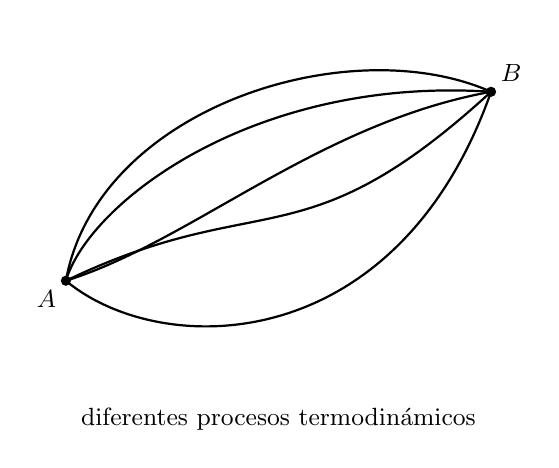
\begin{tikzpicture}
  \coordinate (A) at (0,0); \coordinate (B) at (5.4,2.4);
  \draw[line width=0.8pt] (A) .. controls (0.4,2.2) and (3.6,3.2) .. (B);
  \draw[line width=0.8pt] (A) .. controls (2.5,1.2) and (3.0,0.2) .. (B);
  \draw[line width=0.8pt] (A) .. controls (1.2,-1.0) and (4.2,-1.0) .. (B);
  \draw[line width=0.8pt] (A) .. controls (1.6,0.5) and (3.2,2.0) .. (B);
  \draw[line width=0.8pt] (A) .. controls (0.3,1.0) and (2.4,2.6) .. (B);
  \node[punto] at (A) {}; \node[punto] at (B) {};
  \node[below left] at (A) {$A$}; \node[above right] at (B) {$B$};
  \node[below] at (2.7,-1.5) {diferentes procesos termodinámicos};
\end{tikzpicture}
\end{document}
